\documentclass{article}

\usepackage[english]{babel}
\usepackage[letterpaper,top=2cm,bottom=2cm,left=3cm,right=3cm,marginparwidth=1.75cm]{geometry}
\usepackage{amsmath}
\usepackage{graphicx}
\usepackage[colorlinks=true, allcolors=blue]{hyperref}
\usepackage{listings}
\usepackage{pythontex}
\usepackage{color}
\definecolor{dkgreen}{rgb}{0,0.6,0}
\definecolor{gray}{rgb}{0.5,0.5,0.5}
\definecolor{mauve}{rgb}{0.58,0,0.82}
\lstset{frame=tb,
  language=python,
  aboveskip=3mm,
  belowskip=3mm,
  showstringspaces=false,
  columns=flexible,
  basicstyle={\small\ttfamily},
  numbers=none,
  numberstyle=\tiny\color{gray},
  keywordstyle=\color{blue},
  commentstyle=\color{dkgreen},
  stringstyle=\color{mauve},
  breaklines=true,
  breakatwhitespace=true,
  tabsize=3
}



\title{Statistical Learning: Customer Segments}
\author{Thi Thuy Le - S0564314}

\begin{document}
\fontsize{13pt}{18pt}\selectfont
\maketitle

\tableofcontents
 \vspace{7cm}
\section{Introduction}

\subsection{What is Customer Segments?}


Customer segmentation is the process of dividing customers into groups based on common characteristics so companies can market to each group effectively and appropriately.

A customer segmentation always has a concrete goal, e.g. to better understand customer groups, to create selections for marketing campaigns or to estimate potential. The customer segment is created on the basis of one- or multi-dimensional information that is relevant to the achievement of the goal.

\begin{figure}[htp]
    \centering
    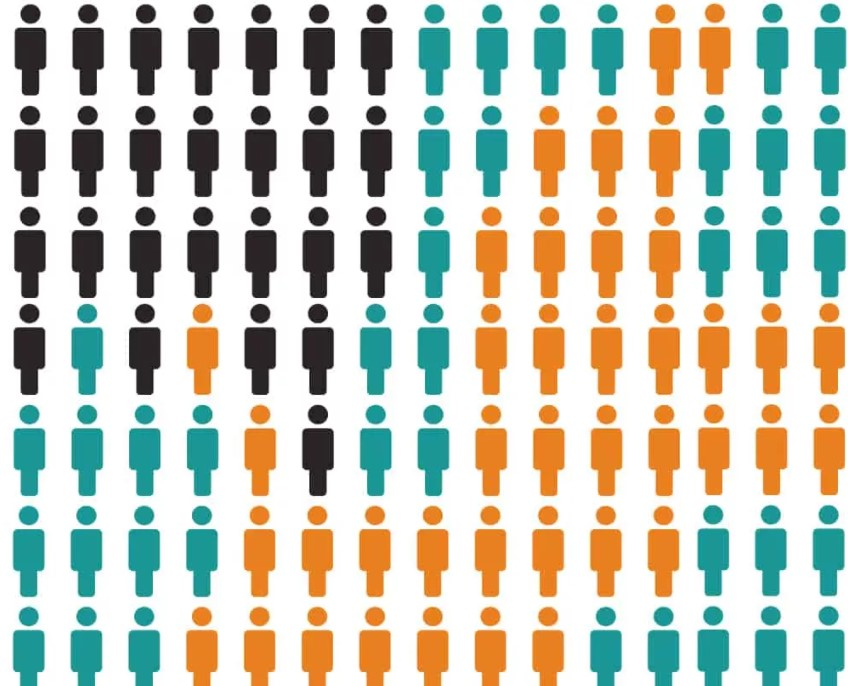
\includegraphics[width=6cm]{Customer.jpg}
    \caption{Customer Segments}
    \label{fig:Customer}
\end{figure}


\subsection{Why is customer segmentation important?}
\begin{itemize}

\item Firstly, identify the right potential customers: Customer segmentation helps the company to identify and understand the characteristics of the target customer, thereby effectively supporting marketing strategies to the target audience. Customers have appropriate age groups, geographical locations, gender, purchasing habits or interests.

\item Second, discover new opportunities in the market: It can be said that customer segmentation is also the basis for marketers to identify and evaluate the market at different times, thereby monitoring progress of the market, predicting the next possible changes in the market in order to anticipate the needs of the market.

\item Third, create specific and relevant messages: By segmenting customers, you can clearly understand what each segment needs from you and from there can create messages that directly address their problems. encountered.

\item Fourth, improve brand loyalty: When customers feel that your products and services are right for them at the right time in their lives, they are more likely to stick with your brand. and recommend it to others.

\item Fifth, make a difference compared to competitors: Companiescan give specific messages to each customer segment, making the brand more prominent and imprinted in the hearts of customers.

\end{itemize}

\section{Data analysis}

Sources we use: \href{https://www.kaggle.com/shwetabh123/mall-customers}{https://www.kaggle.com/shwetabh123/mall-customers}\\
Github: \href{https://github.com/ThiThuyLe/Project-Statistical-Learning}{https://github.com/ThiThuyLe/Project-Statistical-Learning}

\subsection{Data sets}

\textbf{CustomerID}: Unique ID assigned to the customer.\\
\textbf{Gender}: Gender of the customer.\\
\textbf{Age}: Age of the customer.\\
\textbf{Annual Income (k\$)}: Annual Income of the customer.\\
\textbf{Spending Score}: Score assigned by the mall based on customer behavior and spending nature.
\vspace{0,5cm}

First I will include all the important and required Python libraries
Import modules and existing data from Excel into Python. 

\begin{lstlisting}
import matplotlib.pyplot as plt
import numpy as np
import pandas as pd
import seaborn as sns
import sklearn.metrics as sm
from collections import Counter
from sklearn.cluster import KMeans
from pandas import DataFrame
from sklearn.cluster import AgglomerativeClustering
\end{lstlisting}


Then we give a quick reference. And this is what the Dataframe I need to create looks like.

\begin{lstlisting}
df.head()
\end{lstlisting}

\vspace{0,5cm}

\begin{center}
    \begin{tabular}{|l|l|l|l|l|}
    \hline
        CustomerID & Genre & Age & Annual income (k\$) & Spending score (1-100) \\ \hline
        0001 & male & 19 & 15 & 39 \\ \hline
        0002 & male & 21 & 15 & 81 \\ \hline
        0003 & female & 20 & 16 & 6 \\ \hline
        0004 & female & 23 & 16 & 77 \\ \hline
        0005 & female & 31 & 17 & 40 \\ \hline
 \end{tabular}
 \end{center}

\subsection{Check MissingValues NaN}

In order for all data to run smoothly, I have to check if any data is missing.

\begin{figure}[htp]
    \centering
    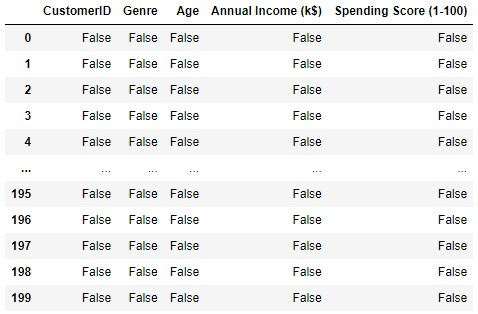
\includegraphics[width=8cm]{MissingValue.jpg}
    \caption{Check MissingValues}
    \label{fig:MissingValue}
\end{figure}

\begin{lstlisting}
df.isnull().sum()
\end{lstlisting}

\begin{figure}[htp]
    \centering
    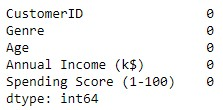
\includegraphics[width=8cm]{MissingValue1.jpg}
    \caption{Sum of the MissingValues}
    \label{fig:Sum of the MissingValues }
\end{figure}

Here it can be seen that there are no missing values.

\subsection{Mean, Min, Max, Median, Standard Deviation of data}

\begin{lstlisting}
df.describe()
\end{lstlisting}

\begin{figure}[htp]
    \centering
    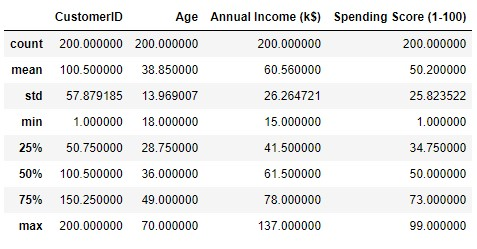
\includegraphics[width=8cm]{Min, Max.jpg}
    \caption{Mean, Min, Max, Median, Standard Deviation of data}
    \label{fig:Mean, Min, Max, Median, Standard Deviation of data}
\end{figure}

Standard deviation of Annual Income and Spending Score are higher than Age.
They can contribute to cluster formation. 

\section{Visualizing data}

\subsection{Annual Income}
\begin{lstlisting}
fig = plt.figure(figsize = (20, 10))
plt.subplot(1, 2, 1)
sns.set(style = 'whitegrid')
sns.distplot(df['Annual Income (k$)'])
plt.title('Distribution of Annual Income', fontsize = 22)
plt.xlabel('Range of Annual Income')
plt.ylabel('Count of Annual Income')

plt.show()
\end{lstlisting}

\begin{figure}[htp]
    \centering
    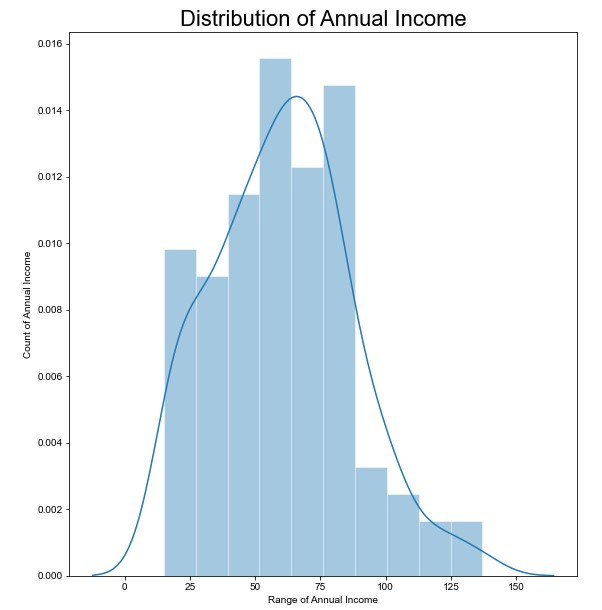
\includegraphics[width=8cm]{Distribution of Annual Income.jpg}
    \caption{Distribution of Annual Income}
    \label{fig:Distribution of Annual Income}
\end{figure}

While in histogram mode, it is also possible to add a KDE (Kernal Density Estimation) curve.

This Annual Income parameter has a maximum value of 137 and a minimum value of 15. The maximum distribution is at the value 70.

The blue lines represent the normal distribution. The distribution of Annual Income is right-skewed and normally distributed. 

\begin{displaymath}
f(x) = \frac{1}{\sigma\sqrt{2\pi}} 
  \exp\left( -\frac{1}{2}\left(\frac{x-\mu}{\sigma}\right)^{\!2}\,\right)
\end{displaymath}

We have a more detailed look at this chart (Figure 6).
\begin{lstlisting}
fig = plt.figure(figsize = (20, 10))
sns.countplot(df['Annual Income (k$)'], palette = 'rainbow')
plt.title('Distribtuion of Annual Income', fontsize = 22)

plt.show()
\end{lstlisting}
\begin{figure}[htp]
    \centering
    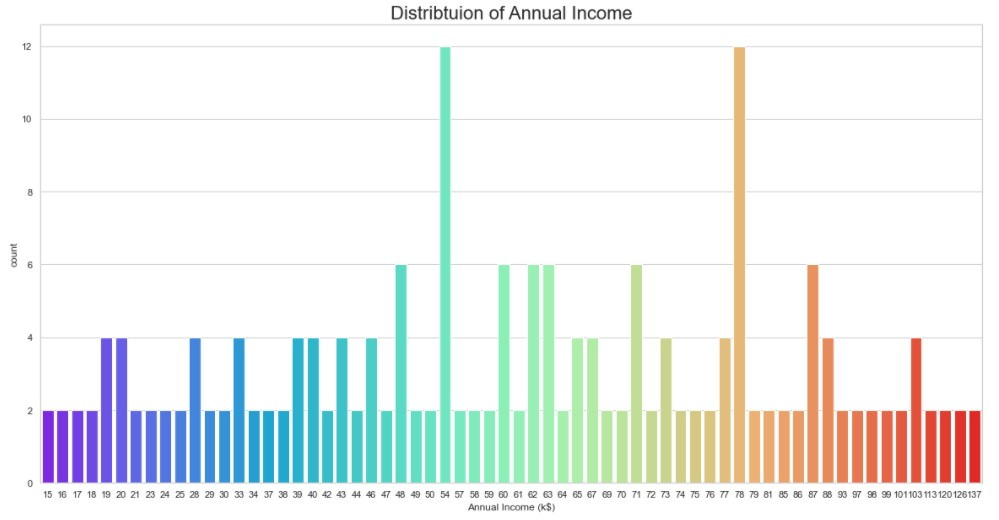
\includegraphics[width=18cm]{Distribution of Annual Income (1).jpg}
    \caption{Distribution of Annual Income}
    \label{fig:Distribution of Annual Income}
\end{figure}

There are many people earning at 54(k\$) and 78(k\$).  

\subsection{Age}

\begin{lstlisting}
fig = plt.figure(figsize = (20, 10))
plt.subplot(1, 2, 2)
sns.set(style = 'whitegrid')
sns.distplot(df['Age'], color = 'green')
plt.title('Distribution of Age', fontsize = 22)
plt.xlabel('Range of Age')
plt.ylabel('Count of Age')

plt.show()
\end{lstlisting}
\vspace{10cm}
\begin{figure}[htp]
    \centering
    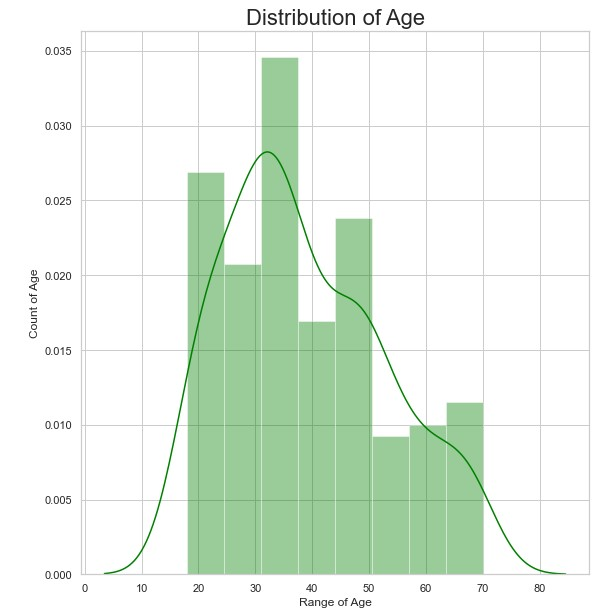
\includegraphics[width=8cm]{Age.jpg}
    \caption{Distribution of Age}
    \label{fig:Distribution of Age}
\end{figure}


This Age parameter has a maximum value of 70 and a minimum value of 18. The maximum distribution is between 30 and 35.
Through this we can also see, the majority of customers are young people. 

We have a more detailed look at this chart (Figure 8).
\begin{lstlisting}
fig = plt.figure(figsize = (20, 10))
sns.countplot(df['Age'], palette = 'rainbow')
plt.title('Distribtuion of Age', fontsize = 22)

plt.show()
\end{lstlisting}
\begin{figure}[htp]
    \centering
    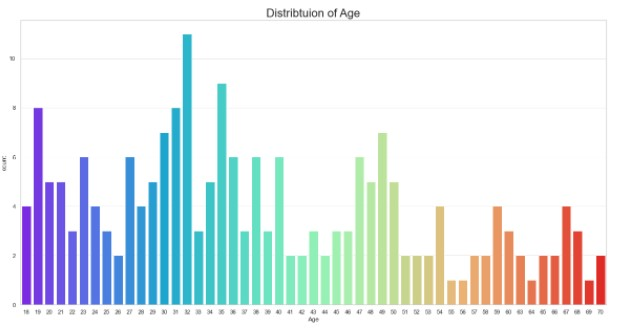
\includegraphics[width=15cm]{Age (1).jpg}
    \caption{Distribution of Age}
    \label{fig:Distribution of Age}
\end{figure}


\subsection{Spending Score (1-100)}

\begin{lstlisting}
fig = plt.figure(figsize = (20, 10))
plt.subplot(1, 2, 2)
sns.set(style = 'whitegrid')
sns.distplot(df['Spending Score (1-100)'], color = 'brown')
plt.title('Distribution of Spending Score (1-100)', fontsize = 22)
plt.xlabel('Range of Spending Score (1-100)')
plt.ylabel('Count of Spending Score (1-100)')

plt.show()
\end{lstlisting}

\begin{figure}[htp]
    \centering
    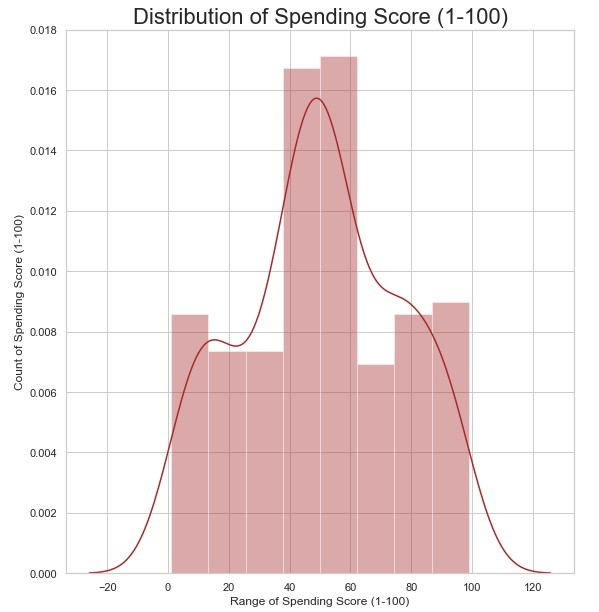
\includegraphics[width=8cm]{Spending Score.jpg}
    \caption{Distribution of Spending Score}
    \label{fig:Distribution of Spending Score}
\end{figure}


This Spending Score parameter has a maximum value of 99 and a minimum value of 1. The maximum distribution is between 40 and 50 and average is 50,20.

If we take a deep dive into the features, it is observed that spending score has 3 peaks(0-20,40-60,80-100)
\vspace{7cm}


We have a more detailed look at this chart (Figure 10).
\begin{lstlisting}
fig = plt.figure(figsize = (20, 10))
sns.countplot(df['Spending Score (1-100)'], palette = 'rainbow')
plt.title('Distribtuion of Spending Score (1-100)', fontsize = 22)

plt.show()
\end{lstlisting}

\begin{figure}[htp]
    \centering
    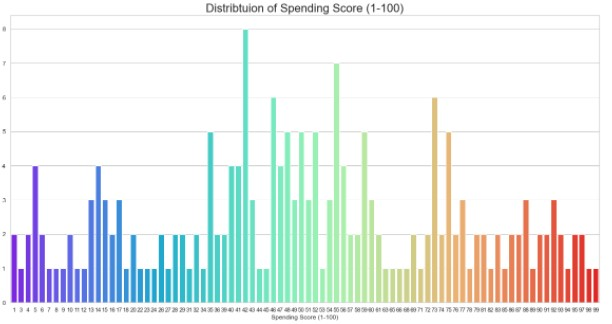
\includegraphics[width=18cm]{Spending Score (1).jpg}
    \caption{Distribution of Spending Score}
    \label{fig:Distribution of Spending Score}
\end{figure}

Most people have an average score.
Those with low or high scores are very few. 
\subsection{Gender}

\begin{lstlisting}
labels= ['Female', 'Male']
size= df['Genre'].value_counts()
plt.rcParams['figure.figsize'] = (6,6)
plt.pie(size, labels=labels,autopct='%1.1f%%')
plt.title('Distribution of Gender', fontsize = 20)
plt.legend()
plt.show()
\end{lstlisting}
\vspace{5cm}
\begin{figure}[htp]
    \centering
    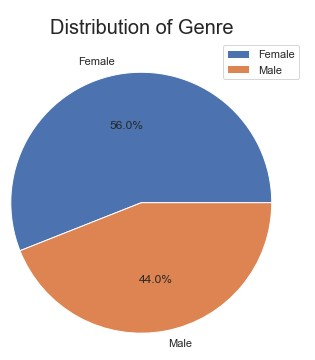
\includegraphics[width=8cm]{Gender.jpg}
    \caption{Distribution of Gender Score}
    \label{fig:Distribution of Gender}
\end{figure}



We divide the Gender into 2 groups. Women make up the majority with 56\% and men with 44\%. In this pie chart we can easily see that women have more passion for shopping than men.\\

\vspace{2cm}
\textbf{Compare between Gender and parameters}

\begin{figure}[htp]
    \centering
    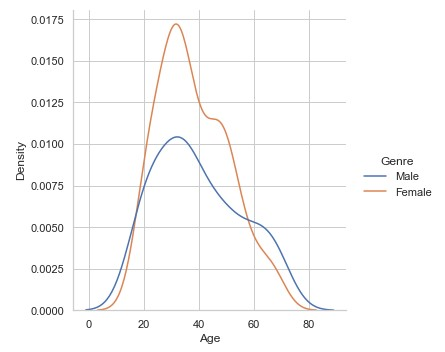
\includegraphics[width=8cm]{Gender vs Age.jpg}
    \caption{Compare Gender vs Age}
    \label{fig:Compare Gender vs Age}
\end{figure}


\begin{figure}[htp]
    \centering
    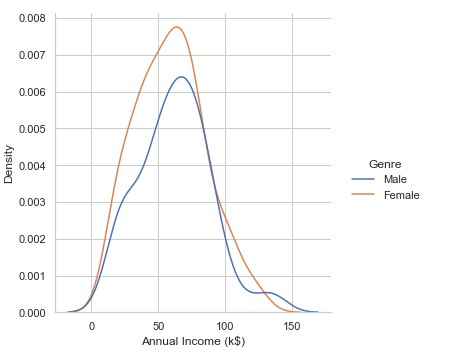
\includegraphics[width=8cm]{Gender vs Annual Income.jpg}
    \caption{Compare Gender vs Annual Income}
    \label{fig:Compare Gender vs Annual Income}
\end{figure}

\begin{figure}[htp]
    \centering
    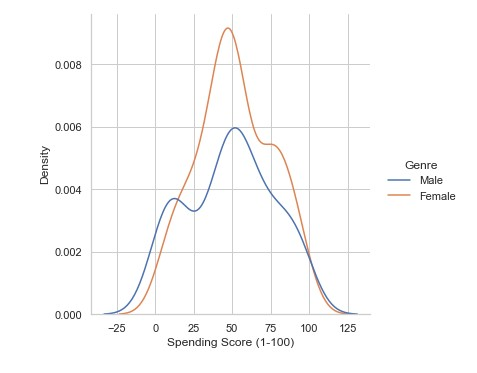
\includegraphics[width=8cm]{Gender vs Spending Score.jpg}
    \caption{Compare Gender vs Spending Score}
    \label{fig:Compare Gender vs Spending Score}
\end{figure}

\vspace{2cm}

Through 3 charts (Figur 12, Figur 13, Figur 14), we can see, the percentage of women is higher than men in all aspects such as Annual Income, Age and Spending Score. 

\vspace{2cm}
\textbf{Compare between Annual Income and Age and Spending Score}
\begin{figure}[htp]
    \centering
    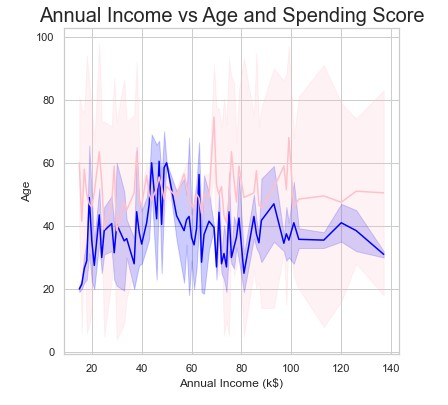
\includegraphics[width=8cm]{Compare.jpg}
    \caption{Compare between Annual Income and Age and Spending Score}
    \label{fig:Compare between Annual Income and Age and Spending Score}
\end{figure}

The above Plot Between Annual Income and Age represented by a blue color line, and a plot between Annual Income and the Spending Score represented by a pink color. shows how Age and Spending Score varies with Annual Income.

\subsection{Correlations of the variables}

First, we want to get an overview of the correlations of the dataset's features. From the plot data it can be seen that between some features from the data is sightly correlated.

\begin{figure}[htp]
    \centering
    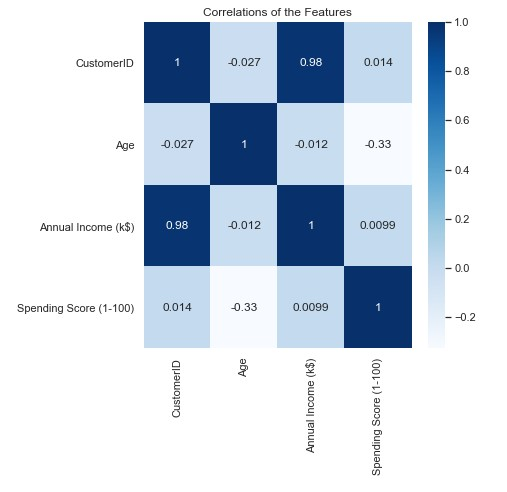
\includegraphics[width=8cm]{Corellation.jpg}
    \caption{Correlations of the variables}
    \label{fig:Correlations of the variables}
\end{figure}
\vspace{5cm}
\section{Clustering Methode}
\subsection{K-Means}
\textbf{Definition}:
K-Means algorithm is a calculation method that can be used for grouping objects, the so-called cluster analysis.
\subsection{Elbow Method}
\textbf{Definition}:
In cluster analysis, the elbow method is a heuristic used in determining the number of clusters in a data set. The method consists of plotting the explained variation as a function of the number of clusters, and picking the elbow of the curve as the number of clusters to use. The same method can be used to choose the number of parameters in other data-driven models, such as the number of principal components to describe a data set.\\
\vspace{6cm}

We will use the elbow method to check the optimal number of clusters.
\begin{lstlisting}
inertias = []
for i in range(1, 11):
    km = KMeans(n_clusters=i).fit(feature)
    inertias.append(km.inertia_)
    
plt.plot(range(1, 11), inertias, 'bx-')
plt.xlabel('Values of K')
plt.ylabel('Inertia')
plt.title('The Elbow Method using Inertia')
plt.show()
\end{lstlisting}
\begin{figure}[htp]
    \centering
    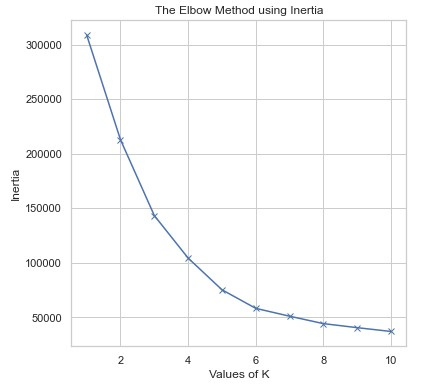
\includegraphics[width=8cm]{Elbow.jpg}
    \caption{Elbow Method}
    \label{fig:Elbow Method}
\end{figure}

From the diagram we can see that 5 is the optimal number of K.\\

We divide customer segments into 5 groups.
\begin{lstlisting}
km = KMeans(n_clusters=5).fit(feature)
y_km = km.fit_predict(feature)
n_cluster, km_count = np.unique(y_km, return_counts=True)
plt.bar(n_cluster, km_count)
plt.ylabel('No of customer')
plt.xlabel('Clustering')
plt.title('Customer segmentation by 5 groups')
\end{lstlisting}

\begin{figure}[htp]
    \centering
    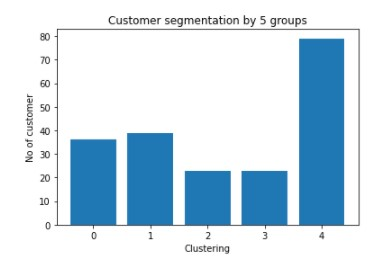
\includegraphics[width=8cm]{Clusters1.jpg}
    \caption{Customer Segmentation by 5 groups}
    \label{fig:Customer Segmentation by 5 groups}
\end{figure}

\vspace{5cm}

Through the chart (Figur 19), we can analyze the following:
\begin{itemize}

\item \textbf{Cluster 1:} The customers have average annual income as well as average spending score.

\item \textbf{Cluster 2:}The customers have lower spending score but have a high annual income.

\item \textbf{Cluster 3:}The customers have lower annual income and lower spending score.
\item \textbf{Cluster 4:} The customers with lower annual income but higher spending score.

\item \textbf{Cluster 5:} The customers have both higher annual income and higher spending score 

\begin{lstlisting}
plt.scatter(X[y_kmeans == 0, 0], X[y_kmeans == 0, 1], s = 100, c = 'orange', label = 'Cluster 1')
plt.scatter(X[y_kmeans == 1, 0], X[y_kmeans == 1, 1], s = 100, c = 'brown', label = 'Cluster 2')
plt.scatter(X[y_kmeans == 2, 0], X[y_kmeans == 2, 1], s = 100, c = 'red', label = 'Cluster 3')
plt.scatter(X[y_kmeans == 3, 0], X[y_kmeans == 3, 1], s = 100, c = 'black', label = 'Cluster 4')
plt.scatter(X[y_kmeans == 4, 0], X[y_kmeans == 4, 1], s = 100, c = 'lightpink', label = 'Cluster 5')
plt.scatter(kmeans.cluster_centers_[:, 0], kmeans.cluster_centers_[:, 1], s = 300, c = 'yellow', label = 'Centroids')
plt.title('Clusters of customers')
plt.xlabel('Annual Income (k$)')
plt.ylabel('Spending Score (1-100)')
plt.legend()
plt.show()
\end{lstlisting}

\begin{figure}[htp]
    \centering
    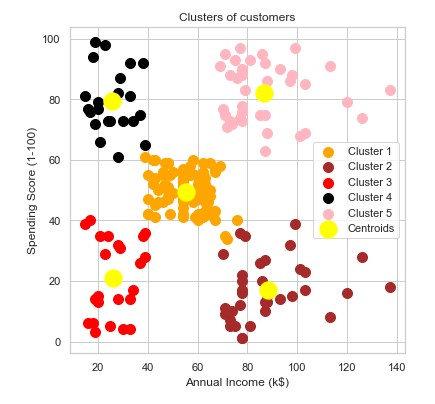
\includegraphics[width=15cm]{Clusters.jpg}
    \caption{Clusters of customers}
    \label{fig:Clusters of customers}
\end{figure}

\end{itemize}

\vspace{5cm}
\section{Summary}
K-means clustering is a type of unsupervised learning, it is usually used when we don't know their groups/categories. The algorithm assign each data point to one of K-groups based on the features similarity.

It is useful to find groups which have not been explicitly labeled in the data. This can be used to confirm business assumptions about what types of groups exist or to identify unknown groups in complex data sets.

\section{Source}
\begin{enumerate} 


\item \href{https://www.kaggle.com/shwetabh123/mall-customers}{https://www.kaggle.com/shwetabh123/mall-customers}
\item Lecture script (Dr. Alla Petukhina)
\item \href{https://www.kaggle.com/shwetabh123/mall-customers/code}{https://www.kaggle.com/shwetabh123/mall-customers/code}
\item \href{https://www.shopify.com/encyclopedia/customer-segmentation}{https://www.shopify.com/encyclopedia/customer-segmentation}
\item \href{https://datasolut.com/kundensegmentierung/}{https://datasolut.com/kundensegmentierung/}
\item \href{https://hedima.vn/journey/tai-sao-cac-cong-ty-nen-phan-khuc-khach-hang/}{https://hedima.vn/journey/tai-sao-cac-cong-ty-nen-phan-khuc-khach-hang/}
\item \href{https://translate.google.com}{https://translate.google.com}
\item \href{https://de.wikipedia.org/wiki/Cluster_(Datenanalyse)}{https://de.wikipedia.org/wiki/Cluster_(Datenanalyse)}
\item \href{https://de.wikipedia.org/wiki/K-Means-Algorithmus}{https://de.wikipedia.org/wiki/K-Means-Algorithmus}
\item \href{https://www.analyticsvidhya.com/blog/2019/08/comprehensive-guide-k-means-clustering/}{https://www.analyticsvidhya.com/blog/2019/08/comprehensive-guide-k-means-clustering/}
\item \href{https://www.youtube.com/watch?v=r-uOLxNrNk8&t=1772s}{https://www.youtube.com/watch?v=r-uOLxNrNk8&t=1772s}
\item Bild \href{https://datasolut.com/kundensegmentierung/}{https://datasolut.com/kundensegmentierung/}
\end{enumerate}


Declaration of Authorship

We hereby confirm that we have authored this Seminar paper independently and without use of others than the indicated sources. All passages (and codes) which are literally or in general matter taken out of publications or other sources are marked as such.

Berlin, 27.02.2022
\vspace{3cm}


Thi Thuy Le

\end{document}
